\documentclass{article}
\usepackage{nameref,hyperref}
\newcommand{\beginsupplement}{%
	\setcounter{table}{0}
	\renewcommand{\thetable}{S4-\arabic{table}}%
	\setcounter{figure}{0}
	\renewcommand{\thefigure}{S4-\arabic{figure}}%
}
\beginsupplement
\usepackage{lastpage,fancyhdr,graphicx}
\newcommand{\ops}{\textsc{ops}}
\newcommand{\opsi}{O\textsc{ps}}
\newcommand{\vcps}{\textsc{vcps}}
\newcommand{\owl}{\textsc{owl}}
\newcommand{\owli}{O\textsc{wl}}
\newcommand{\sparql}{\textsc{s}par\textsc{ql}}
\newcommand{\bfo}{\textsc{bfo}}
\newcommand{\dbpedia}{\textsc{db}pedia}
\newcommand{\foaf}{\textsc{foaf}}
\newcommand{\ict}{\textsc{ict}}
\newcommand{\html}{\textsc{html}}
\newcommand{\node}{\textsc{n}ode.js}
\newcommand{\facebook}{\textsc{f}acebook}
\newcommand{\twitter}{\textsc{t}witter}
\newcommand{\wwwc}{\textsc{w3c}}
\newcommand{\skos}{\textsc{skos}}
\newcommand{\etherpad}{\textsc{e}therpad}
\newcommand{\ogp}{\textsc{ogp}}
\newcommand{\iri}{\textsc{iri}}
\newcommand{\uri}{\textsc{uri}}
\newcommand{\urii}{U\textsc{ri}}
\newcommand{\urll}{\textsc{url}}
\newcommand{\ngo}{\textsc{ngo}}
\newcommand{\http}{\textsc{http}}
\newcommand{\opa}{\textsc{op}a}
\newcommand{\ocd}{\textsc{ocd}}
\newcommand{\ontologiaa}{\textsc{o}ntologiaa}
\newcommand{\obs}{\textsc{obs}}
\newcommand{\pubby}{\textsc{p}ubby}
\newcommand{\rdf}{\textsc{rdf}}
\newcommand{\mysql}{\textsc{m}y\textsc{sql}}
\newcommand{\aan}{\textsc{aa}}
\newcommand{\cidadedemocratica}{\textsc{c}idade \textsc{d}emocr\'atica}
\newcommand{\participa}{\textsc{p}articipa.br}
\newcommand{\ontop}{\textsc{o}n\textsc{t}op}
\newcommand{\quest}{\textsc{q}uest}
\newcommand{\webprotege}{\textsc{w}ebprotege}
\newcommand{\obda}{\textsc{obda}}
\newcommand{\pnud}{\textsc{undp}}
\newcommand{\onu}{\textsc{un}}
\newcommand{\vbs}{\textsc{vbs}}
\newcommand{\lod}{\textsc{lod}}
\newcommand{\corais}{\textsc{c}orais}
\newcommand{\serpro}{\textsc{s}erpro}
\newcommand{\python}{\textsc{p}ython}
\newcommand{\protege}{\textsc{p}rot\`eg\`e}

\usepackage[margin=1em]{geometry}
\begin{document}
Public consultations have core importance in participatory democracy and the model in Figure~\ref{fig:consult} was conceived as part of \vcps\ community documentation.
An \owl\ implementation of such public consultation was meant to be developed and made public, with dedicated attention.
Considerations of this public consultation with respect to the \ops\ and formal existent instances was envisioned as well.
This public consultation model is observed here for completeness of exposition and further details goes beyond the scope of this article. A public consultations along the lines of a recent Presidential decree~\cite{decree} was formalized in \obs\ \owl\ and in \vbs\ \skos~\cite{pnud5}.

\begin{figure*}[H]
    \centering
    \vspace{-.35cm}
    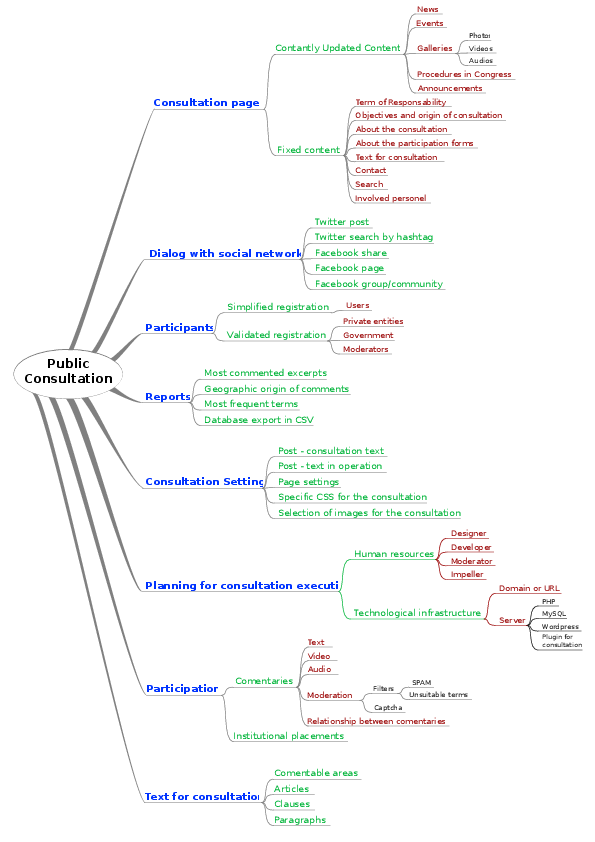
\includegraphics[width=0.9\textwidth]{../figs/publicConsultation__}
    \caption{A diagram representation of a general public consultation, part of initial \vcps\ documentation.}
    \label{fig:consult}
\end{figure*}
\bibliography{../plos}
\bibliographystyle{plain}



\end{document}
